\documentclass{article}
\usepackage[utf8]{inputenc}
\usepackage{multicol}
\usepackage{mathpazo}
\usepackage{textcomp}
\usepackage{amsmath}
\usepackage{mdframed}
\usepackage{xcolor}
\usepackage{hyperref}
\usepackage{graphicx}
\usepackage[landscape=true]{geometry}

 \geometry{
 left=20mm,
 right=20mm,
 }

\definecolor{astral}{RGB}{176, 224, 230}
\definecolor{lred}{HTML}{EFAAAA}

\title{\textbf{Computational Biology}}
\author{Gian Hiltbrunner}
\date{January 2020}

\begin{document}

\begin{multicols*}{3}


\maketitle
\vspace{-0.7cm}
\begin{mdframed}[backgroundcolor=lred] 
    \textbf{Disclaimer}\\
    Parts of the information provided within this document may be incomplete and/or incorrect.\\For corrections please submit a pull request to:
    \url{http://github.com/protelescristata/SummaryComputationalBiology}
\end{mdframed}

\section{Models of Molecular Evolution}
\subsection{Substitution Rate Matrices}

\subsubsection{JC69}
\begin{itemize}
    \item  All substitutions have the same rate $\lambda$
    \item 1 parameter
\end{itemize}

\begin{center}
    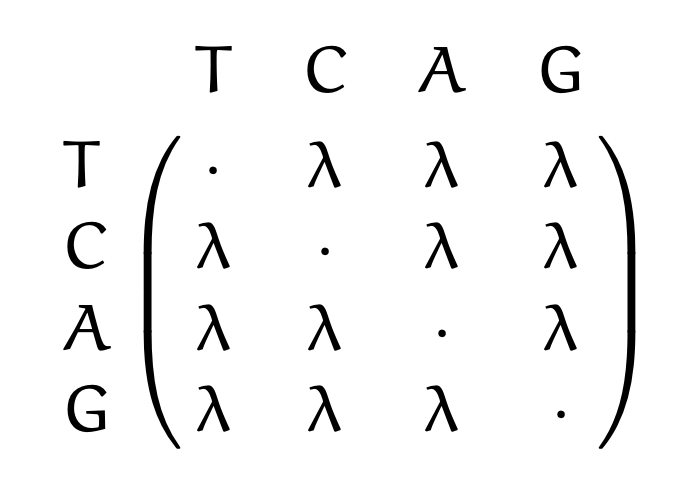
\includegraphics[width=0.5\linewidth]{js69.png}
\end{center}

\subsubsection{K80}
\begin{itemize}
    \item This model differentiates between transitions (T-C/A-G) and transversions. 
    \item 2 parameters
\end{itemize}

\begin{center}
    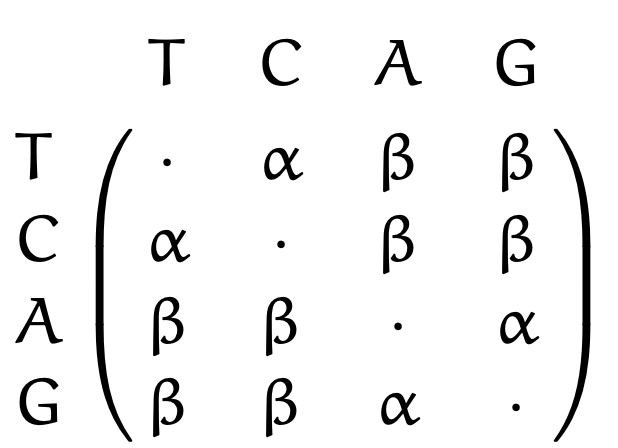
\includegraphics[width=0.5\linewidth]{k80.png}
\end{center}

\subsubsection{TN93}
\begin{itemize}
    \item Transitions between T/C happen with rate $\alpha_1 \times \pi$
    \item Transitions between A/G happen with rate $\alpha_2 \times \pi$
    \item Transversions happen with rate $\beta\times \pi$
    \item 3 + 3 ($\pi_x$) parameters 
\end{itemize}

\begin{center}
    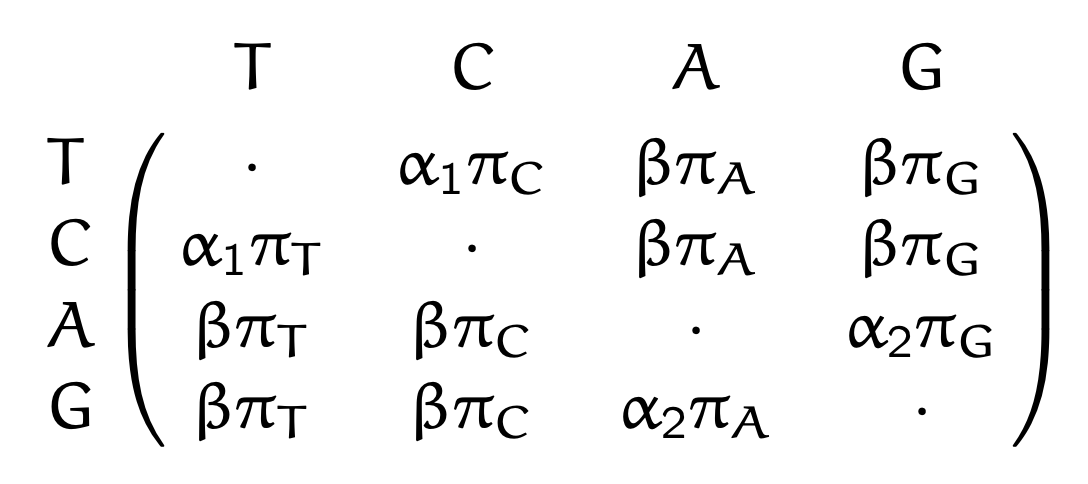
\includegraphics[width=0.7\linewidth]{tn93.png}
\end{center}

\begin{itemize}
    \item If $\alpha_1 = \alpha_2$, the model is named \textbf{HKY}
\end{itemize}

\subsubsection{GTR - Generalised Time Reversible}

\begin{itemize}
    \item[+] quite flexible
    \item[+] time-reversible
    \item[-] not completely general
    \item 6 + 3 ($\pi_x$) parameters 
\end{itemize}

\begin{center}
    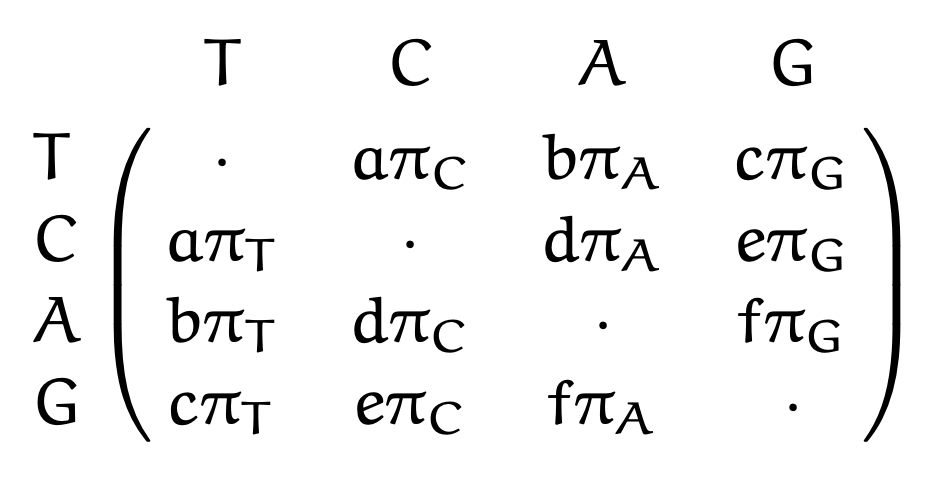
\includegraphics[width=0.7\linewidth]{GTR.png}
\end{center}
\subsubsection{UNREST}

\begin{itemize}
    \item Unrestricted model 
    \item Each substitution has a different rate
    \item[+] Most general model 
    \item[+] Other models are special cases of UNREST
    \item[-] Mathematically complicated to handle
    \item[-] Not time-reversible
    \item 12 parameters 
\end{itemize}

\begin{center}
    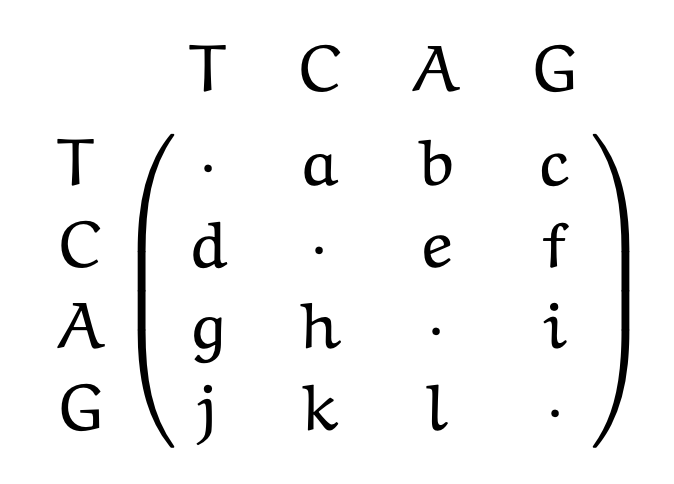
\includegraphics[width=0.5\linewidth]{unrest.png}
\end{center}

\subsection{Calculating Sequence Distance}
\subsubsection{Transition Probability Matrix}
\label{transprobmat}

Using the substitution rate matrix $Q$ we derive the transition probability matrix $P(t)$, which gives the probabilities of nucleotide $i$ changing to nucleotide $j$ in any time interval $t$.

\begin{center}
    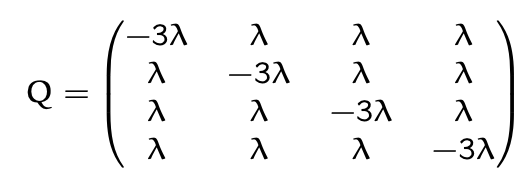
\includegraphics[width=0.5\linewidth]{substitutionratematrix.png}
\end{center}

$$P(t) = \text{e}^{Qt}$$

\begin{center}
    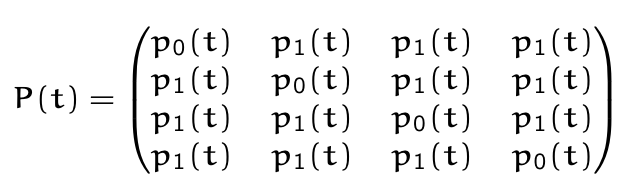
\includegraphics[width=0.7\linewidth]{transitionprobabilitymatrix.png}
\end{center}

\subsubsection{Stationary Distribution}

\begin{itemize}
    \item For $t \rightarrow \infty$ we reach a stationary distribution; where the transition probabilities all tend towards $0.25$. 
    \item Any long sequence will thus be composed of equal amounts of T,C,A and G at $t \rightarrow \infty$
\end{itemize}

\subsection{Maximum Likelihood Estimators}
\begin{mdframed}[backgroundcolor=astral] 
    \textbf{Likelihood Function}\\
    Describes a hypersurface whose peak represents the combination of model parameter values that maximize the probability of drawing the obtained sample. 
\end{mdframed}

\begin{mdframed}[backgroundcolor=astral] 
    \textbf{Maximum Likelihood Estimator}\\
    Is an estimator of a model parameter that maximises the probability to obtain the observed results.
\end{mdframed}

\textbf{Example}: Estimate the probability that a die shows side 6. $\rightarrow$ The die is thrown $n = 100$ times and we obtained a 6 $x = 40$ times. 
\begin{itemize}
    \item Define probability of throwing a 6 $x$ times out of $n$ tries $\rightarrow$ Binomial-distribution, thus: $P = {n\choose x}p^x(1-p)^{n-x}$, where $p$ is the probability of throwing a 6
    \item We use this probability as our likelihood function and plug in the given values: $L(p;x) = {100\choose 40}p^{40}(1-p)^{60}$
    \item To find the maximum likelihood we calculate the first derivative of our likelihood function and set $L' = 0$ to find the maximum. 
    \item Transformations are sometimes applied to the likelihood function. e.g.: $l(p;x) = \log (L(p;x))$
    \item We estimate the probability by solving for $p$ and get $p = 0.4 \neq 1/6$
\end{itemize}

\subsubsection{Confidence Intervals}

Interval which tries to capture the uncertainty of a parameter estimate. 

\begin{mdframed}[backgroundcolor=astral] 
    \textbf{Confidence Interval}\\
    If a parameter is repeatedly estimated from realisations of the random experiment and the interval estimate for each realisation, we expect 95 \% of these intervals to contain the true parameter.
\end{mdframed}

Confidence intervals may be calculated on the basis of likelihood intervals.\\
Let $X$ be a random variable with a distribution parametrised in $\theta$. Based on collected data $x$ of a huge sample, the maximum likelihood estimation for the parameter is $\hat{\theta}$. Then, $2(l(\hat{\theta} - l(\theta)) \sim x^2_k$
\begin{itemize}
    \item Determine the value of the log likelihood function in $\hat{\theta}$: $l(\hat{\theta};x)$
    \item Calculate $l(\hat{\theta};x) - 0.5x^2_{k,5\%}$; subtract half of the $5\%$ most extreme values according to the $x^2$-distribution
    \item Determine those $\theta$ values for which the the following holds: 
    $l(\theta;x) = l(\hat{\theta};x) - 0.5x^2_{k,5\%}$
\end{itemize}

\subsubsection{MLE for Sequence Distance}
The MLE framework can be used to derive a maximum likelihood estimation for the sequence distance under a JC69 model. 
We have the transition probability matrix as seen in subsection (\ref{transprobmat}) with:
\begin{align*}
    p_0(t) = \frac{1}{4} + \frac{3}{4}\text{e}^{-4\lambda t}\\
    p_1(t) = \frac{1}{4} + \frac{1}{4}\text{e}^{-4\lambda t}
\end{align*}
For two sequences of length $n$ with $x$ differences the probability that any one position is different is $p = 3p_1(t)$. We define $d = 3\lambda t$ as the expected distance in time $t$ and get for the probability that $x$ out of $n$ positions are different: \begin{align*}
L(d;x) = {n \choose x} p^{x}(1-p)^{n-x}=\\
{n \choose x}
\left(\frac{3}{4}-\frac{3}{4} e^{-\frac{4}{3} d}\right)^{x}\left(\frac{1}{4}+\frac{3}{4} e^{-\frac{4}{3} d}\right)^{n-x}
\end{align*}
\begin{itemize}
    \item We compute $l(d;x) = \log(L(d;x))$
    \item An calculate the first derivative $\hat{d} = l'(d;x)$⁄⁄
\end{itemize}

Which gives us the MLE of the JC69 distance: 
$$\hat{d} = -\frac{3}{4}\log\left(1-\frac{4x}{3n}\right)$$

\subsubsection{Example of JC69 MLE}

\begin{center}
    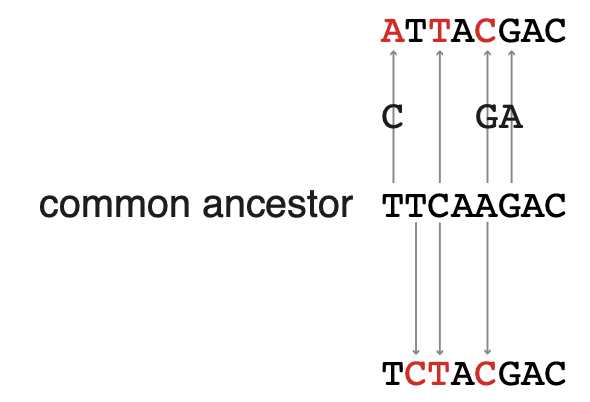
\includegraphics[width=0.5\linewidth]{mlejc69.png}
\end{center}

\begin{itemize}
    \item Length of gene: $n = 8$
    \item Differences between the two sequences: $x = 2$
\end{itemize}

$$\hat{d} = -\frac{3}{4}\log\left(1-\frac{4\times 2}{3\times 8}\right) = 0.3$$
Determine the $95 \%$ confidence interval for the given parameters. 

\subsection{Variable Substitution Rates}

\begin{itemize}
    \item Not all sites evolve at the same rate
    \item Mutation rates may vary across sites \item The acting selection in the phenotypic level exerts different evolutionary pressure on different sites
\end{itemize}

\section{Cladistic and ML Inference}
{\color{red} MISSING CONTENT PP5-6; Here beigins PP7}

\subsection{Searching Tree Space}
To search the tree space for the maximum likelihood tree we need to propose different trees for evaluation. 
\begin{itemize}
    \item We propose different unrooted trees using various defined moves to alter the tree
    \item We propose trees with different branch lengths; thus we multiply each branch length by some factor
\end{itemize}
$\rightarrow$ We can then use "hill-climbing" strategies to find the ML tree

\subsubsection{Modifying Unrooted Trees}

\begin{itemize}
    \item \textbf{Nearest-Neighbour Interchange (NNI)}: Swap two subtrees of opposing sides of one branch. 
    \item \textbf{Suptree Pruning and Regrafting (SPR)}: Remove one random subtree and attach at a random position of the tree.
    \item \textbf{Branch swapping by tree bisection and reconnection (TBR)}: Cut the tree into two and reconnect at random by selecting branches on both trees and connecting the subtrees between them. 
\end{itemize}

\subsection{Model Testing}

Here we introduce methods for model selection and assessing the confidence of our parameters. 

\subsubsection{Likelihood Ratio Testing}

\begin{itemize}
    \item Consider two models: $H_1$ as a general model parameterised in $\theta_0$ and $H_1$ as a nested model parameterised in $\theta_0$.
    \item Derive the likelihood function for both models and the maximum likelihood estimators $\hat{\theta_0}$ and $\hat{\theta_1}$ for given dataset. 
    \item Compute if $2(\log L (\hat{\theta_1}) - \log L(\hat{\theta_0}))$ is in the $\alpha$ tail of $x_{df}^2$, then reject the null model $H_0$   
\end{itemize}

\begin{mdframed}[backgroundcolor=astral] 
    \textbf{Likelihood Ratio Test}\\
    Is used to assess the goodness of fit of two models based on the ratio of their likelihoods. One model is found by maximizing the likelihood over the whole parameter space while the other is evaluated under some constraints. If the constraint (hypothesis) is supported by the data the likelihoods should not differ significantly.
\end{mdframed}

\subsubsection{Testing Non-Nested Models}

\textbf{Akaike Information Criterion (AIC)}: Used for testing non-nested models:
$$\text{AIC} = -2\log L_i(\hat{\theta}_i) + 2p_i$$
where $p_i$ is the number of parameters and $L_i$ the likelihood function of model $i$.

\begin{itemize}
    \item Calculate the AIC for each model
    \item Choose the model with the lowest AIC; thereby minimizing the Kullback-Leibler distance to the true model  
\end{itemize}

Rules of thumb for multiple model comparisons: 
\begin{itemize}
    \item AIC $\leq$ 1-2 + minimum $\rightarrow$ substantial support, should receive consideration in inference
    \item AIC $\leq$ 4-7 + minimum $\rightarrow$ low support
    \item AIC $\geq$ 10 + minimum $\rightarrow$ essentially no support
\end{itemize}

\subsubsection{Confidence Intervals}

Each parameter value which is not rejected based on the likelihood ratio test at the $0.05$ level is within the $95\%$ interval.
$\rightarrow$ Use the strategy as introduced before.
\begin{itemize}
    \item Determine the value of the log likelihood function in $\hat{\theta}$: $l(\hat{\theta};x)$
    \item Calculate $l(\hat{\theta};x) - 0.5x^2_{k,5\%}$; subtract half of the $5\%$ most extreme values according to the $x^2$-distribution
    \item Determine those $\theta$ values for which the the following holds: 
    $l(\theta;x) = l(\hat{\theta};x) - 0.5x^2_{k,5\%}$
\end{itemize}

\subsubsection{Bootstrapping}
\begin{itemize}
    \item Sample $m$ sites at random with replacement
    \item Infer a phylogeny based on the new data
    \item Repeat this procedure many times 
\end{itemize}

\begin{center}
    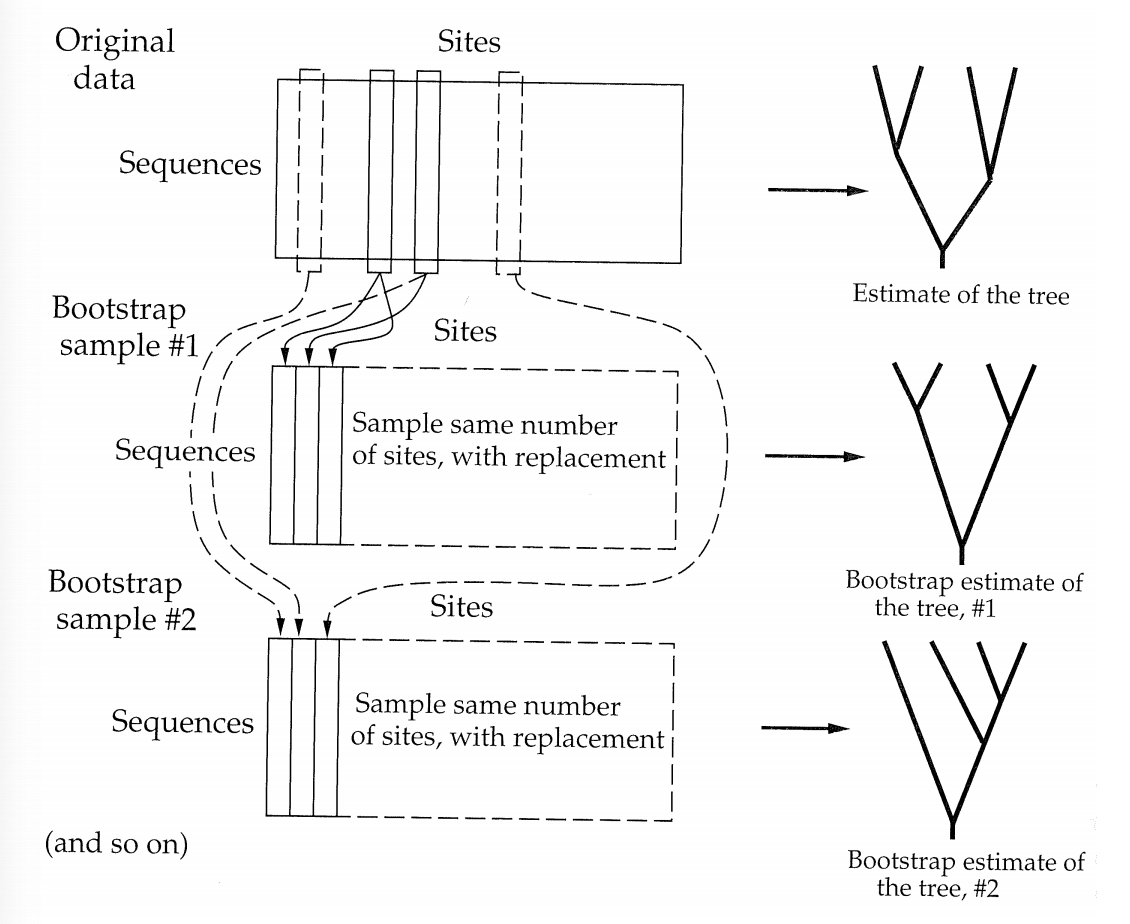
\includegraphics[width=1\linewidth, angle=0.6]{bootstrapping.png}
\end{center}

\subsection{Overview of ML Inference}

\begin{enumerate}
    \item Infer a ML tree 
    \begin{itemize}
        \item Felsenstein's pruning algorithm for each tree and branch length
        \item Choose the tree with branch lengths that optimize the likelihood
        \item Do this for each substitution model and calculate its AIC
    \end{itemize}
    \item Determine the substitution model and tree with highest support using AIC
    \item Determine the confidence interval for the substitution model parameters based on the likelihood ratios
    \item Determine the confidence in your maximum likelihood tree using bootstrapping
\end{enumerate}

\section{Comparative Methods}

\subsection{Comparing Discrete Characters}

Example: We want to know whether eye and hair color are correlated. 

\begin{center}
    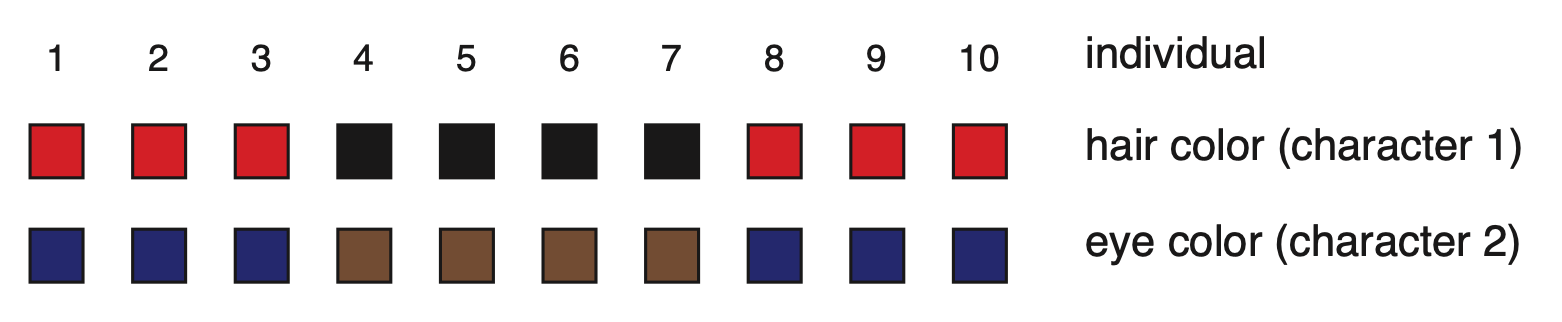
\includegraphics[width=1\linewidth, angle=0.6]{compdischar.png}
\end{center}

To test whether there is a true correlation we perform Fisher's exact test.\\
$H_0$: Having brown eyes is equally likely among red- and black-haired individuals.\\

\begin{tabular}{|l|l|l|}
\hline
\textbf{hair/eyes} & \textbf{brown} & \textbf{blue} \\ \hline
\textbf{red}       & 0              & 6             \\ \hline
\textbf{black}     & 4              & 0             \\ \hline
\end{tabular}

Evaluating the contingency table above yields the following. 
{
\footnotesize
\begin{align*}
P(red/brown) =& \frac{(RBr\ in\ R)\times (BlBr\ in\ Bl)}{Br\ in\ All}\\
=& \frac{{6\choose 0}{4\choose 4}}{{10\choose 4}} = 0.0048 < 0.05
\end{align*}
}
Thus we reject the hypothesis of independent character evolution on the 0.05 significance level, indicating that there is a correlation. 

\textbf{Caveat}: We should consider that there may be a bias due to the relatedness of the individuals. Fisher's exact test assumes independence which may not be given here.\\

\subsubsection{Reformulated Fisher's Test}

Thus we reformulate our problem: \textbf{Is the change of characters on the branches correlated?}

\begin{center}
    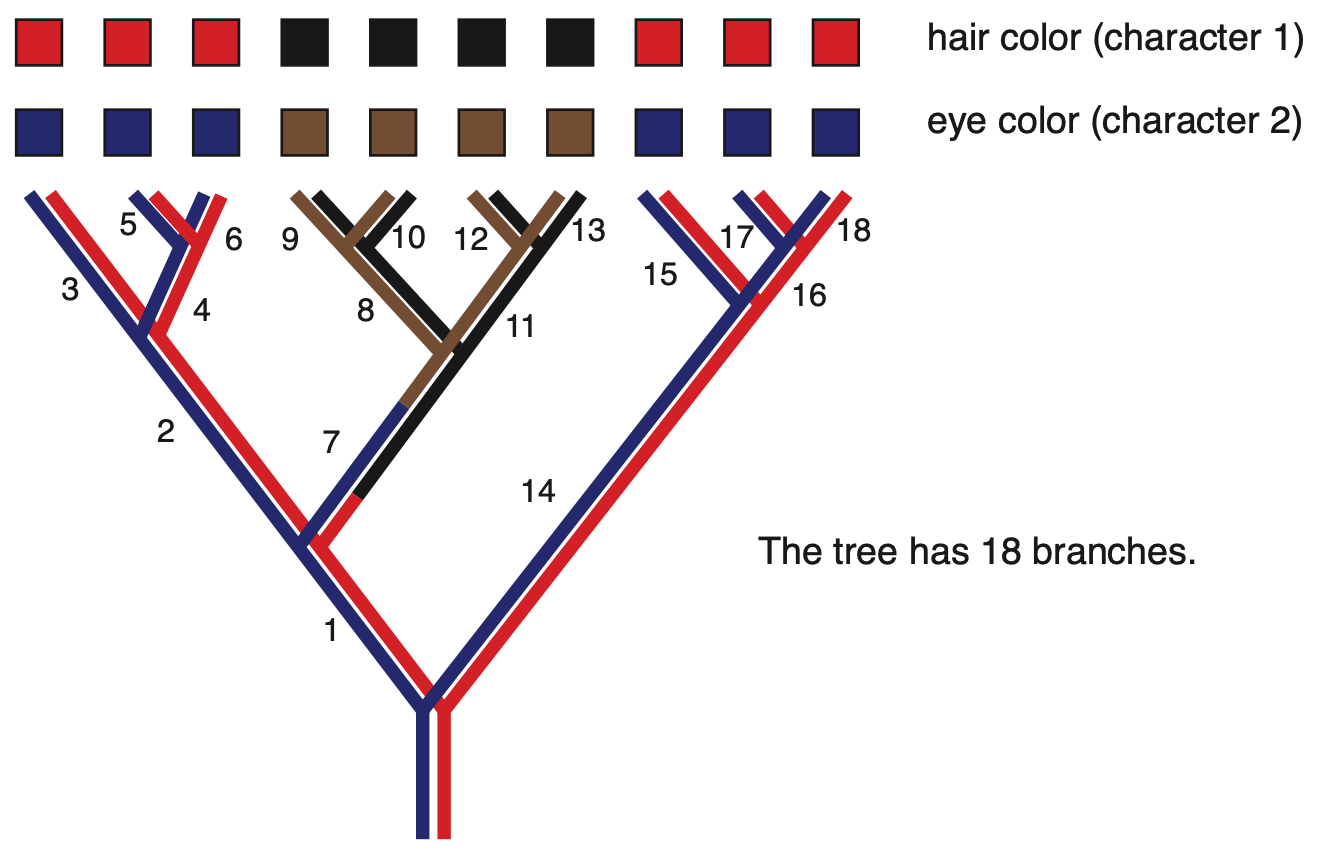
\includegraphics[width=1\linewidth, angle=0.6]{compdischarphylo.png}
\end{center}

$H_{0, new}$: The character changes are equally likely on every branch.\\ 

\begin{tabular}{|l|l|l|}
\hline
\textbf{hair/eyes} & \textbf{yes} & \textbf{no} \\ \hline
\textbf{yes}       & 1              & 0             \\ \hline
\textbf{no}     & 0              & 17             \\ \hline
\end{tabular}\\

This contingency table summarizes on how many branches we have a change in either the hair color, the eye color or both. Here we have \textbf{one} branch with a change in both and \textbf{17} branches with no change.\\

The probability for one branch on which both the hair and eye color changes ($E$) is under $H_{0, new}$:

\begin{align*}
    P(E|H_{0,new}) =& \frac{{1\choose 1}{17\choose 0}}{{18\choose 1}} = 0.05555 > 0.05
\end{align*}

Neglecting the phylogenetic background can lead to false conclusions on correlations between characters, because of non-independence of species data points as a result of shared ancestry.\\

Here we do not consider differences in branch length, but these are important as changes are more likely to happen on longer branches. 

\subsection{Comparing Continuous Characters}

We now switch our focus from discrete characters (e.g. color) to continuous phenotypic characters (e.g. height, weight, virulence). 

\subsubsection{Linear Regression on Phylogenies}

We cannot use linear regression models two compare two characters which evolved on a phylogeny as we cannot distinguish between correlations and clade effects. 

\begin{center}
    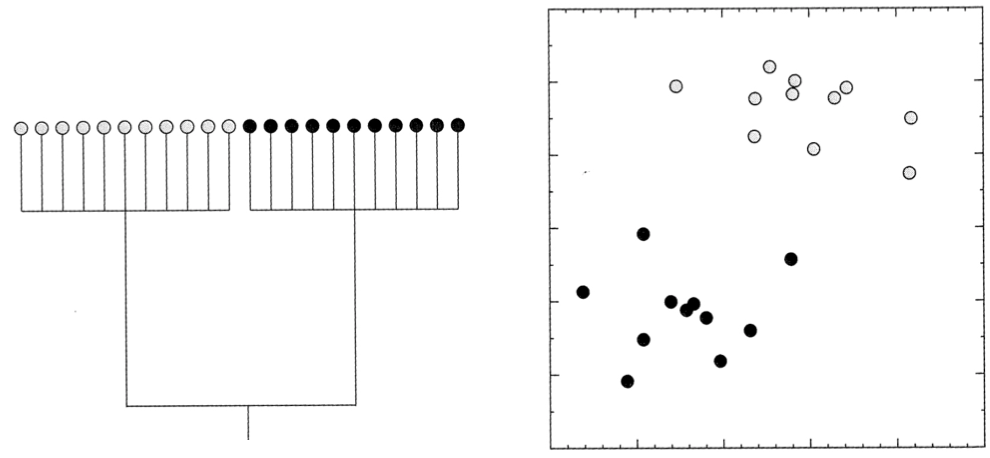
\includegraphics[width=1\linewidth, angle=0.6]{phyloregress.png}
\end{center}

When characters evolve on a tree:

\begin{itemize}
    \item ...they share common evolutionary history and are not independent realisations
    \item ...the variance/error added by Brownian motion is not equally distributed 
\end{itemize}

Thus the prerequisites for linear regression (see: {\color{astral}Linear Regression}) are not given.  
\subsubsection{Brownian Motion}

Brownian motion is a Wiener process and thus follows four conditions: 

\begin{itemize}
    \item $W_0$ = 0, the process start in $0$
    \item $W_t$ is almost surely continuous: $P(W_t$ continuous $) = 1$  
    \item $W_t$ has independant increments (memorylessness): For $0 \seq s_1 \seq t_1 < s_2 \seq t_2$, $(W_{t_1} - W_{s_1})$ and $(W_{t_2} - W_{s_2})$ are independent 
    \item For $0 \leq s \leq t$, the $W_t - W_s \sim N(0,\sigma^2(t-s))$
\end{itemize}

There are analogies between models for evolution on discrete and continuous character space.
\begin{center}
    \begin{tabular}{|l|l|}
\hline
\textbf{discrete}                                                                         & \textbf{continuous}                                                                   \\ \hline
\begin{tabular}[c]{@{}l@{}}probability\\ to visit any\\ state\end{tabular}                & \begin{tabular}[c]{@{}l@{}}probability\\ density on \\ state space\end{tabular}       \\ \hline
\begin{tabular}[c]{@{}l@{}}memory-\\ lessness due\\ to Markov-\\ chain model\end{tabular} & \begin{tabular}[c]{@{}l@{}}memory-\\ lessness due\\ to Brownian\\ motion\end{tabular} \\ \hline
\begin{tabular}[c]{@{}l@{}}transition\\ probabilities\\ scale with \\ time\end{tabular}   & \begin{tabular}[c]{@{}l@{}}variance\\ scales \\ with \\ branch \\ length\end{tabular} \\ \hline
\end{tabular}
\end{center}

Given a phylogeny we can apply a Brownian motion model to evolve a continuous character. 

\begin{center}
    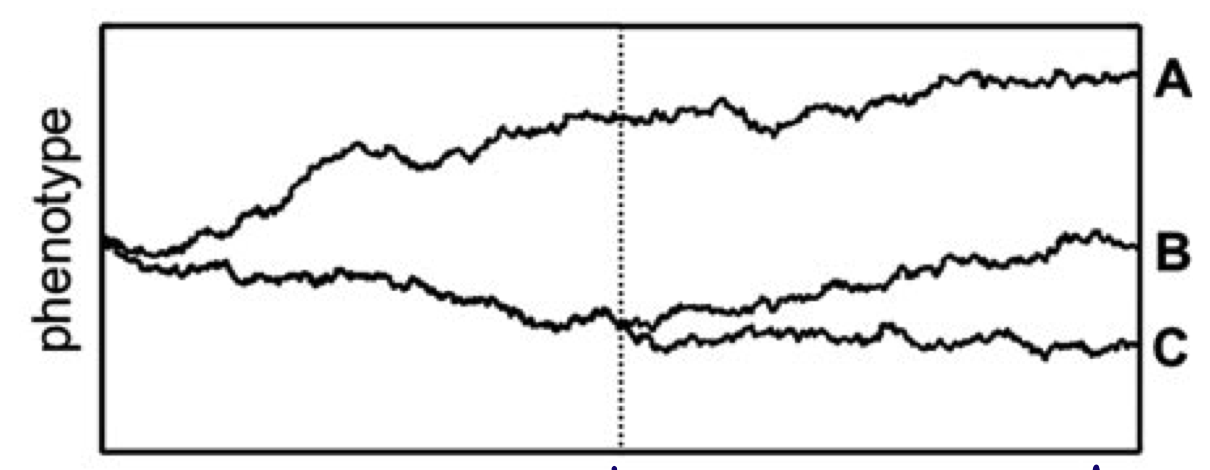
\includegraphics[width=1\linewidth, angle=0.6]{brownphyl.png}
\end{center}

\begin{mdframed}[backgroundcolor=astral] 
    \textbf{Linear Regression}\\
    Determine dependency of a variable $Y$ in another variable $X$. We measure $Y$ and $X$ for $n$ independent realizations and fit a regression model to the data. The observations need to be:
    \begin{itemize}
        \item independent
        \item have the same (normally) distibuted errors
    \end{itemize}
    
    Then we have the model: 
    
    $$y_i = \beta x_i + b + \epsilon, \text{ where } \epsilon \sim N(0, \epsilon^2)$$
    
    This is fit using a least squares method and the goodness of fit is estimated by $R^2$. An $R^2$ of $1$ indicates a perfect fit. 
\end{mdframed}

\end{multicols*}
\end{document}
